\documentclass[a4paper, 10pt, conference]{ieeeconf}    




\usepackage{graphics} % for pdf, bitmapped graphics files
\usepackage{epsfig} % for postscript graphics files
\usepackage{mathptmx} % assumes new font selection scheme installed
\usepackage{times} % assumes new font selection scheme installed
\usepackage{amsmath} % assumes amsmath package installed
\usepackage{amssymb}  % assumes amsmath package installed
\usepackage[export]{adjustbox}
\usepackage{stfloats}

\newcommand*{\Comb}[2]{{}^{#1}C_{#2}}%
\title{\LARGE \bf
Dota2 Game Prediction
}


\author{Yukai Qiao
}


\begin{document}



\maketitle
\thispagestyle{empty}
\pagestyle{empty}


%%%%%%%%%%%%%%%%%%%%%%%%%%%%%%%%%%%%%%%%%%%%%%%%%%%%%%%%%%%%%%%%%%%%%%%%%%%%%%%%
\begin{abstract}

In this paper, we present two machine learning approaches to predict the game result for the popular computer game Dota2 using team composition. The first approach uses a linear model: logistic regression. The second approach uses convolutional neural network with pretrained hero vectors using Word2vec. Results indicate that each approach has its advantages. Logistic regression only learns impacts of individual heroes to games but achieved highest accuracy. While the deep learning model is assumed to learn some interactions between heroes and achived higher F1 score than logistic regression.

\end{abstract}


%%%%%%%%%%%%%%%%%%%%%%%%%%%%%%%%%%%%%%%%%%%%%%%%%%%%%%%%%%%%%%%%%%%%%%%%%%%%%%%%
\section{INTRODUCTION}

Dota2 is one of the most popular online game. It is also the originator of multiplayer online battle arena(MOBA) game. Professional Dota2 tournaments often offer prizes in millions of US dollars in total. The most recent The International tournament has a total prize pool of \$24,787,916\cite{track}.  A predictor of such a game could be further developed to provide strategical analysis to professioanal teams.\\

In a regular game of Dota, there are ten players separated to two sides. Each player can pick one of 113 heroes in the match. The only way for one side to defeat another is to destroy the ``ancient'' of the opponent's team. Players often play in different roles by convention. Each hero has different attribute and unique abilities which decide what roles it is capable of. When players pick heroes they need to consider the combination of roles and heroes, some powerful hero combos and countering enemies' pick. 

An experienced player can often predict the trend or even the result of a match by the composition of both teams --- so called ``draft''. There are certain patterns between the ``draft'' and the result of the match, however, the total amount of the draft of a single team is $\Comb{113}{5}=140364532 $, and the combination of two teams is greater than $1.564\times10^{16}$. The complexity is huge, and machine learning is suitable for solving such a problem.\\

We present two approaches: Logistic regression which outperforms other traditional machine learning methods, and convolutional model combined with pretrained word2vec hero vectors.

\section{Dataset}

Data are collected from 200,000 ranked matches using API provided by valve. Data are split randomly into training set, validation set and test set in ratio of $75\%:12.5\%:12.5\%$


\section{Approaches}

\subsection{Logistic Regression)}

The basic idea of predicting the result of a match is to compare the strength of both teams and a naive solution is to measure the individual strength of each hero and then compare the total sum of strength of both teams. As a linear model, logistic regression is supposed to implement what was proposed.\\

The architecture is similar to Conley and Perry's\cite{conley2013does} work.

The input are the concatenation of two one-hot encoding vectors of both teams.

There are 113 heroes in Dota2 currently, with 2 teams, draft can be represented as a feature vector $x\in\mathbb{R}_{226}$
\[
	x_{i}=\begin{cases}
			1 $ if a hero with id $i$ is in the radiant team,$\\
			0
	    \end{cases}
\]	
\[
	x_{i+113}=\begin{cases}
			1 $ if a hero with id $i$ is in the dire team,$\\
			0
	    \end{cases}
\]	
The output is binary where 1 represents radiant win and 0 represents dire win.\\

\subsection{Convolutional neural network with Word2vec}

\begin{figure*}[b]
	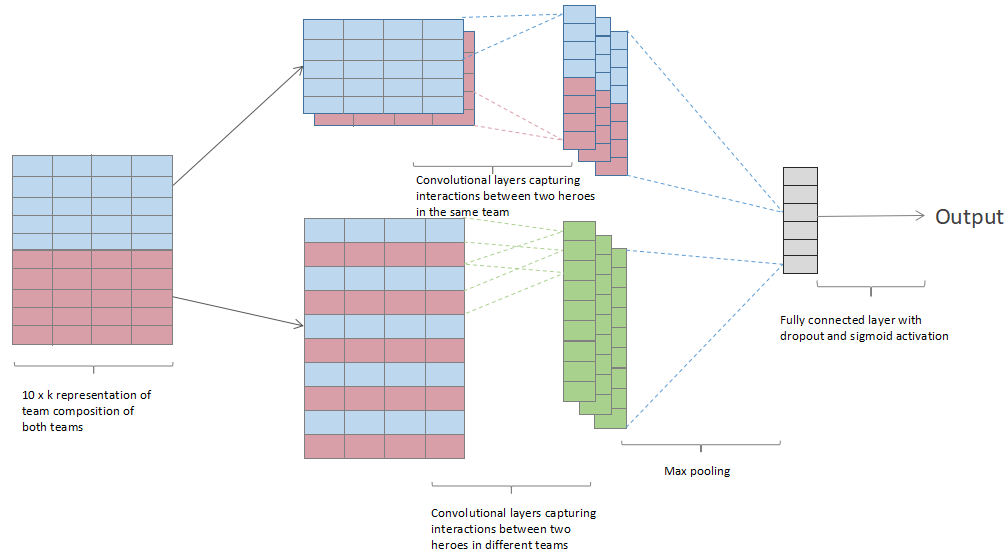
\includegraphics[width=1\textwidth] {architecture.png}
	\caption {The architecture of the model}
\end{figure*}

Inspired by similar approach in natural language processing(NLP) area, we realized that our problem has many similarities with sentence classification. Dota2 players tend to pick a well-structured and balanced team, this implies that heroes with similar role would share a common set of teammates. As for natural language, similar words also share a common context. In game of Dota2, the performance of a team greatly depends on interactions between heroes. The meaning of a sentence also relies on the interactions between words. \\

We developed a model imitating Yoon Kim's\cite{kim2014convolutional} work on sentence classification.

\subsubsection{Word2vec}
There are two ways of implementing Word2vec\cite{mikolov2013efficient}: skip-gram model and negative sampling. Although it was using negative sampling in our implementation, we will explain how it works with skip-gram model, since the theory behind negative sampling is essentially skip-gram model.\\
We are given a corpus of words $w$ and their contexts $c$ within a window size. Given a corpus $Text$, the goal is to derive the parameters $\theta$ to maximize the corpus probability\cite{goldberg2014word2vec}:\\
\begin{center}
$\begin{aligned}
\arg\max_{\theta}\prod_{(w,c)\in D}p(c|w,\theta)
\end{aligned}$
\end{center}
In our case, a word $w$ is a hero, its context $c$ is its teammates. D is the set of all two-hero pairs in the same team. The corpus are all teams in our trainning data. The window size is 4 since we are certain that a hero interacts with all 4 of its teammates.
\subsubsection{Architecture}

The input of the model is a $10\times k$ matrix concatenated from two of $5\times k$ matrices representing the team compositions for both team where each row is a hero vector. Since there is no spatial information in team composition, in other words, the position of a hero in a team doesn't matter, the order of rows of each $5\times k$ matrices are augmented to random permutations at each epoch. \\

As shown in figure 1, the model is split into two parts in the next step. Firstly, both $5\times k$ matrices goes through a shared conv pool layer with filter size of 2 which attempts to capture interactions between heroes in the same team. The output from those two layers are concatenated vertically.\\

Secondly, the input is reordered into staggered arrangement in respect to team and then connect to a conv pool layer. This part of the model is supposed to capture two-hero interactions of different teams.\\

The output of those two parts are concatenated vertically and then connect to a fully connected layer with dropout and sigmoid output.


\section{Result and discussion}
We use accuracy, F1 score and roc auc score as metrics of our models.\\
\begin{table}[h]
\centering
\begin{tabular}{| r| l | l | l |}
	\hline
	 & Accuracy & F1 score & roc auc score \\ \hline
	Conv & 0.5841 & 0.6540 & 0.6151 \\ \hline
	LR & 0.5916 & 0.6456 & 0.6226\\ \hline

\end{tabular}
\caption{Test results of two models}
\end{table}\\
Logistic regression performed slightly better in terms of accuracy and roc auc score, but not F1 score, which means that the conv model achived a better balance between precision and recall. We believe its because logistic regression assumes heroes are not correlated therefore it only learns individual strength, but the strength of a team is not simply the sum of individual strength of heroes. For example, the five heroes with highest winrate don't make a good team because the roles of some of them overlaps and the team would not be balanced. On the other hand, conv model completely ignores individual strength and focuses on interactions between heroes. It is more likely to be aware of roles and the balance of a team. However, people always choose balanced team in the game and they also try hard not to be countered by the opponents. This implies that we don't actually have much data on situations with balanced team vs. imbalanced team or one team is countered hard by the other, which means these features are not producing much predicting power as expected. 

\nocite{*}
\bibliographystyle{ieeetran}
\bibliography{confbib}





\end{document}